\documentclass[11pt]{article}
\usepackage[margin=0.82in]{geometry}
\usepackage{graphicx}
\usepackage{amsmath}
\usepackage{amssymb}
\usepackage{hyperref}
\usepackage{booktabs}
\title{Projected Relations from Prime-Field Hyperelliptic Covers}
\author{Reproducible toy study}
\date{24 October 2026}
\begin{document}
\maketitle
\noindent\textbf{Question.} Can the covers
$C_{d,s}:y^2=f(t^d+s)$ of an elliptic curve $E:y^2=f(x)$ supply
reusable projected relations and blind-target descent with total work
below $\sqrt{\ell}$? This report tests one bounded linear-section
family on a public $\mathbb F_{101}$ fixture. It does not implement
Enge's high-genus Jacobian algorithm or establish an asymptotic bound.

\begin{center}
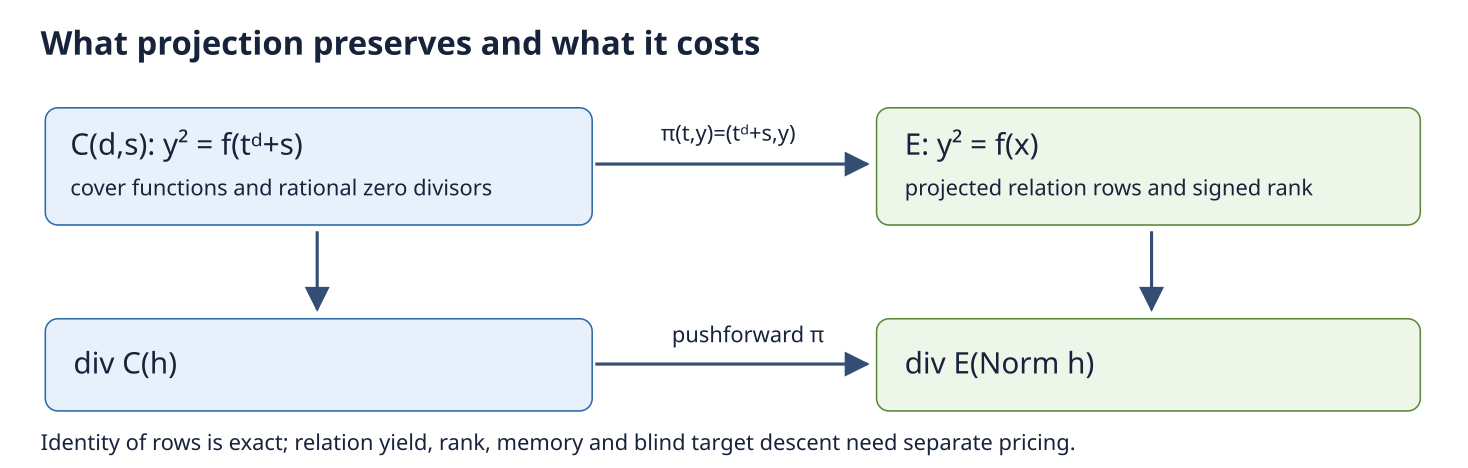
\includegraphics[width=0.96\linewidth]{cover_projection.png}
\end{center}

\section*{Algebraic reduction}
For $p>3$, $d$ prime to $p$, and $f(s)\ne0$, the cover is smooth and
has genus $(3d-1)/2$ for odd $d$ or $(3d-2)/2$ for even $d$.
The degree-$d$ map $\pi(t,y)=(t^d+s,y)$ gives
$\pi_*\pi^*=[d]$ on $E=\operatorname{Jac}(E)$.
The divisor norm identity is
$\pi_*(\operatorname{div}_C h)=\operatorname{div}_E N(h)$.
For $h=y-(at+b)$,
\[
N(h)=(y-b)^d-a^d(x-s).
\]
For the degree-two target section
$h=y-y_Q-(t^2+s-x_Q)(ct+b)$, with
$A=y-y_Q-b(x-x_Q)$, the direct elliptic norm is
\[
N(h)=A^2-c^2(x-s)(x-x_Q)^2.
\]
The degree-two product identity has an evaluated
\texttt{identity.certificate/v1} record and Lean proof source in the
study directory. The Lean build was not verified in this run; the source
does not formalize the geometric norm map.

\section*{Exhaustive public fixture}
The curve is $E/\mathbb F_{101}:y^2=x^3+x+46$, with
$\#E=109$, $G=(2,37)$, and $Q=(64,19)$.
The Rust collector does not take the target scalar as input.
Each cover scans all $101^2$ sections $y-(at+b)$, retaining a row only
when its full finite zero divisor splits into distinct rational points.
Target sections are scanned only when the target fiber is fully rational.
The table gives counts, not timings.

\begin{center}
\begin{tabular}{rrrrr}
\toprule
$(d,s)$ & genus & projected points & full public splits &
signed rank/columns \\
\midrule
$(2,0)$ & 2 & 56 & 30 & 9/25 \\
$(3,0)$ & 4 & 108 & 0 & 0/2 \\
$(5,0)$ & 7 & 20 & 0 & 0/2 \\
$(7,0)$ & 10 & 108 & 0 & 0/2 \\
$(2,6)$ & 2 & 44 & 8 & 2/11 \\
\bottomrule
\end{tabular}
\end{center}

\begin{center}
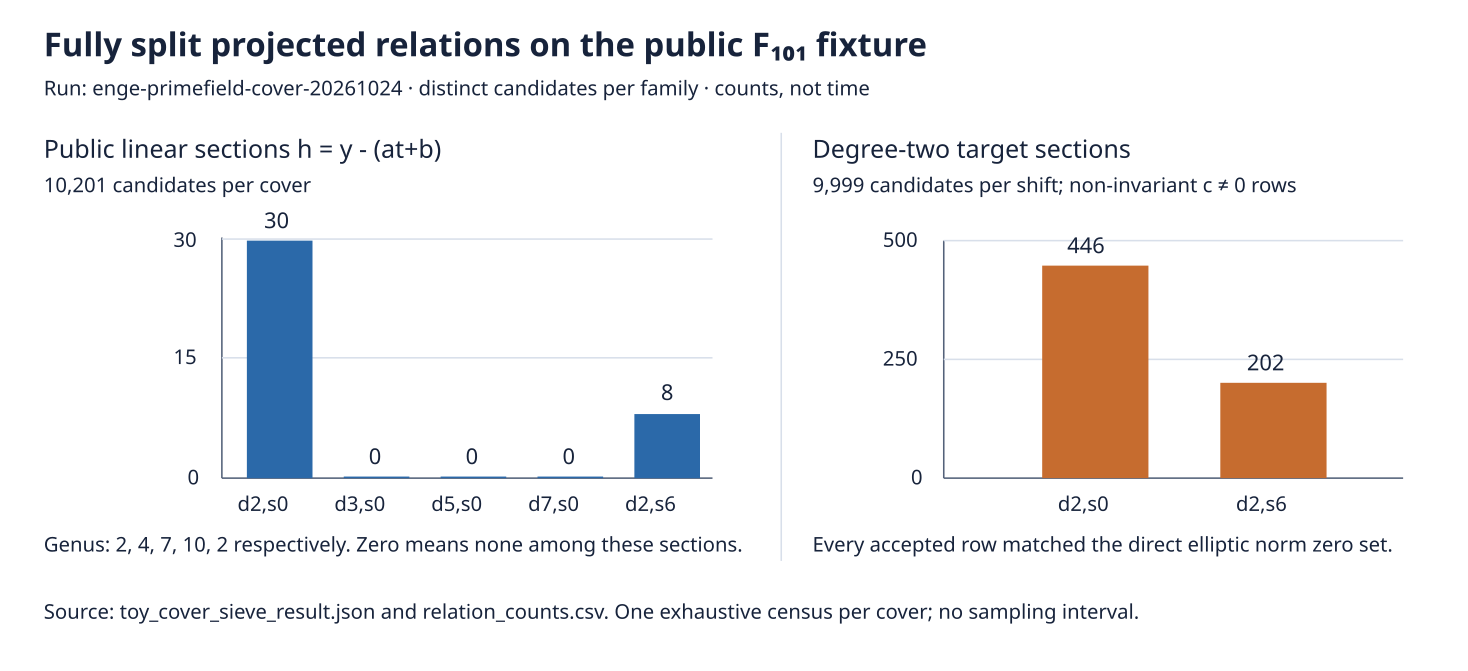
\includegraphics[width=0.97\linewidth]{relation_counts.png}
\end{center}

For $(d,s)=(2,6)$, target-only streaming recovered $\log_G Q=37$
after 1,070 candidate sections, 108,070 cover-point tests, and 22
accepted rows. The signed relation matrix had rank 21 on 22 columns;
anchoring $\log G=1$ determined $\log Q$. A separate multiplication
verified $37G=Q$. Across the full target census, all 202 non-invariant
fully split rows matched the direct elliptic norm zeros, and the same
202 parameter pairs were accepted directly on $E$.

The deterministic rho control reached a collision after 72 elliptic
group operations. Cover-point tests, rank solves, and group operations
are unlike units, so these figures are not a calibrated speed ratio.
The shift $s=6$ was chosen using public $G,Q$; that selection cost was
not measured. No below-rho conclusion follows. At genera 4, 7, and 10,
zero relations were found only within this fully rational linear-section
factor base; higher-degree primes and Enge's full algorithm are untested.

\section*{Replay and status}
The native run record, root result copy, and exact replay commands are
listed in the adjacent \texttt{REPORT.md}. Run the study crate's release
tests and release binary with Cargo.
The collector verifies each accepted row by elliptic addition, each
direct norm zero set, and the recovered scalar by multiplication.
The open next step is a degree-$B>1$ cover-prime factor base with
arbitrary-divisor norm, projected rank, target descent, and one-target
same-host cost and memory accounting.
\end{document}
